\section{Praktischer Teil}
  
  \subsection{Geräteparameter}
    
    In der folgenden Tabelle werden alle relevanten Geräteparameter aufgelistet. 
    
    \begin{table}[H]
      \centering
      \caption[Auflistung der Geräteparameter, Quelle: Autor]{Auflistung der Geräteparameter}
      
      \label{tab:Gerateparameter}
      \begin{tabular}{@{}l|p{7cm}l@{}}
        \toprule
        Parameter & Beschreibung \\ \midrule
          HPLC System & Agilent 1100 Series \\
          Software & Chemstation von Agilent \\
          Säule & ACE HPLC-Säule EXCEL 3 C18-PFP, Pentaflourophenyl \\ 
          Länge der Säule & \SI[mode=text]{150}{\milli\meter} \\
          Innendurchmesser der Säule & \SI[mode=text]{4.6}{\milli\meter} \\
          Mobile Phasen & Eluent A: Wasser (Milli-Q Anlage) mit \SI[mode=text]{0.1}{\percent} TFA, Eluent B: Acetonitril (HiPerSolv CHROMANORM, HPLC Super Gradient) \\ 
          Eluentenzusammensetzung & isokratisch, \SI[mode=text]{55}{\percent} Eluent B \\
          Flussrate & \SI[mode=text]{1.0}{\milli\liter\per\minute} \\
          Druck & 177-\SI[mode=text]{178}{bar} \\
          Temperatur & \SI[mode=text]{40}{\degreeCelsius} \\
          Injektionsvolumen & \SI[mode=text]{20}{\micro\liter} \\
          Detektoreinstellungen & DAD, detektiert bei \SI[mode=text]{230}{\nano\meter} \\ 
          Totzeit inkl. Bestimmung & Thioharnstoff wird in 1:1 Methanol/Wasser gemischt und gemessen - $t_0 = \SI[mode=text]{1.452}{\minute}$ \\ \bottomrule
      \end{tabular}
    \end{table}
  
  \subsection{Chemikalienliste} \label{sec:Chemikalien}
  
    In Tabelle \ref{tab:Chemikalien} befindet sich eine Auflistung der verwendeten Chemikalien, die für die qualitative und quantitative Analyse verwendet wurden. Die Strukturen der Chemikalien sind in Abbildung \ref{fig:Strukturen} dargestellt. Für die verwendeten Laufmittel sind keine Daten bekannt. 
    
      \begin{table}[H]
        \centering
        \caption[Auflistung der verwendeten Chemikalien, Quelle: Autor]{Auflistung der verwendeten Chemikalien.}
      
        \label{tab:Chemikalien}
        \begin{tabular}{@{}l|llllp{4.5cm}l@{}}
          \toprule
          Chemikalie & CAS Nummer & Reinheit & $M$ in \si{\gram\per\mole} & Lieferant \\ \midrule
           Carbamazepin (Analyt)  & 298-46-4 & $\geq \SI[mode=text]{99}{\percent}$ (HPLC) & \SI[mode=text]{236.27}{\gram\per\mole} & SIGMA \\
           Ibuprofen (Analyt)  & 15687-27-1 & $\geq \SI[mode=text]{98}{\percent}$ (GC) & \SI[mode=text]{206.29}{\gram\per\mole} & SIGMA \\
           Naproxen (Analyt) & 22204-53-1 & Reference Material & \SI[mode=text]{230.26}{\gram\per\mole} & SIGMA \\
           Estron (Analyt) & 53-16-7 & $\geq \SI[mode=text]{99}{\percent}$ & \SI[mode=text]{270.37}{\gram\per\mole} & SIGMA \\
           Estradiol (Analyt) & 50-28-2 & $\geq \SI[mode=text]{98}{\percent}$ & \SI[mode=text]{272.38}{\gram\per\mole} & SIGMA \\ \bottomrule
        \end{tabular}
      \end{table}
    
      \begin{figure}[H]
        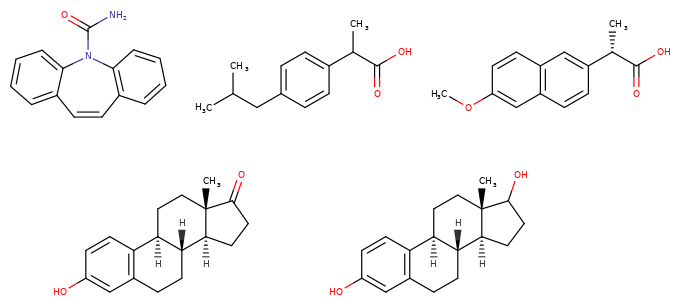
\includegraphics[scale=0.45, center]{images/Structures.png} 
        \caption[Strukturen der verwendeten Chemikalien, Quelle: Autor]{Strukturen der verwendeten Chemikalien: Carbamazepin, Ibuprofen, Naproxen, Estron, Estradiol (von links nach rechts, links oben beginnend).}
        \label{fig:Strukturen}
      \end{figure}
    
    
  \subsection{Bestimmung einer optimalen Eluentenzusammensetzung}
  
    Die verwendeten Lösungsmittel sind \SI[mode=text]{0.1}{\percent}-ige Triflouressigsäure (TFA) in Wasser (Eluent A) und Acetonitril (Eluent B). Vor Verwendung werden die beiden Laufmittel im Ultraschallbad entgast. Ein Online-Entgaser in der HPLC entfernt die letzten Gasreste, damit diese die Trennung nicht stören. Folgende Laufmittelzusammensetzungen wurden getestet:
    
      \begin{enumerate}
        \item \SI[mode=text]{30}{\percent} Eluent B, Flussrate \SI[mode=text]{1.0}{\milli\liter\per\minute}
        \item \SI[mode=text]{55}{\percent} Eluent B, Flussrate \SI[mode=text]{1.0}{\milli\liter\per\minute}
        \item \SI[mode=text]{55}{\percent} Eluent B, Flussrate \SI[mode=text]{0.5}{\milli\liter\per\minute}
        \item \SI[mode=text]{70}{\percent} Eluent B, Flussrate \SI[mode=text]{1.0}{\milli\liter\per\minute}
      \end{enumerate}
    Die Probe mit den 5 Analyten Carbamazepin, Ibuprofen, Naproxen, Estron und Estradiol wird aufgegeben und nach Einstellen der Laufmittelzusammensetzung die Analyse gestartet. Auf diese Weise werden alle oben angegebenen Laufmittelzusammensetzungen getestet. Vor jeder Änderung der Zusammensetzung wird das System für mind. \SI[mode=text]{5}{min} äquilibriert. Bei der optimalen Laufmittelzusammensetzung wird die Totzeit durch Injektion einer Lösung von Thioharnstoff (Detektion bei \SI[mode=text]{254}{\nano\meter}) bestimmt. \\
    
    Es zeigt sich, dass die zweite Laufmittelzusammensetzung (\SI[mode=text]{55}{\percent} Eluent B, Flussrate \SI[mode=text]{1.0}{\milli\liter\per\minute}) die beste Trennung der Substanzen liefert. Bei der ersten Laufmittelzusammensetzung (bezogen auf obenstehende Tabelle) sind die Retentionszeiten viel zu groß, da im Prinzip nur der erste Eluent sichtbar ist. Die anderen Eluenten sind nach Ende der Analyse also vermutlich noch in der Säule. Bei der vierten Laufmittelzusammensetzung kommt es zu einer Überlappung zweier benachbarter Peaks, was eine Trennung unmöglich macht. Bei der dritten Laufmittelzusammensetzung sind zwar alle Peaks schön getrennt, jedoch braucht die letzte Substanz doppelt so lang wie bei der zweiten Laufmittelzusammensetzung. Aus diesen Gründen wird bei den Folgenden Analysen die zweite Laufmittelzusammensetzung verwendet.
    
  \subsection{Qualitative und quantitative Bestimmung von Wasserrückständen nach der Methode des externen Standards}
    
    Für die qualitative Bestimmung wird ein Chromatogramm von jeder Substanz aufgenommen. Aus diesen Chromatogrammen bestimmt man die für eine Substanz charakteristische  Retentionszeit und den  Kapazitätsfaktor. Anschließend wird die Probe gemessen, die Peaks durch Vergleich der Kapazitätsfaktoren zugeordnet und weitere chromatographische Parameter bestimmt. \\
    
    Für die quantitative Bestimmung werden für jede der in \ref{sec:Chemikalien} angeführten Chemikalien \SI[mode=text]{100}{\milli\liter} einer \SI[mode=text]{500}{ppm} Urstandardlösung hergestellt. Dazu werden je \SI[mode=text]{50}{\milli\gram} von Carbamazepin, Ibuprofen, Naproxen, Estron und Estradiol in einen \SI[mode=text]{100}{\milli\liter} Messkolben eingewogen und bis zur Marke aufgefüllt. \SI[mode=text]{20}{\milli\liter} der jeweiligen Urstandardlösung werden entnommen und in einen \SI[mode=text]{100}{\milli\liter} Messkolben transferiert. Aufgefüllt wird mit einem Gemisch aus \SI[mode=text]{70}{\percent} Methanol und \SI[mode=text]{30}{\percent} Wasser, das auf 50:50 verdünnt wird. Ausgehend von dieser \SI[mode=text]{100}{ppm} Standardlösung werden Standardlösungen mit 10, 20, 30, 40 und \SI[mode=text]{50}{ppm} hergestellt. Damit das Gesamtvolumen immer \SI[mode=text]{1}{\milli\liter} beträgt werden 0.1, 0.2, 0.3, 0.4 und \SI[mode=text]{0.5}{\milli\liter} des \SI[mode=text]{100}{ppm} Standards mit der Kolbenhubpipette entnommen und auf \SI[mode=text]{1}{\milli\liter} aufgefüllt. Um die eben angegeben Volumina zu berechnen, wird die Verdünnungsformel
    
      \begin{equation}
        V_1 = \frac{V_2 c_2}{c_1}
      \end{equation}  
    verwendet. Die hergestellten Standardlösungen werden jeweils dreimal gemessen und eine Kalibriergerade mithilfe der Peakfläche erstellt. Anschließend wird die Probelösung dreimal gemessen und  aus der Kalibriergerade die Konzentration der einzelnen Substanzen bestimmt. 
    
      \begin{table}[H]
      \centering
      \caption[Übersicht zur Herstellung der Kalibrierstandard-Lösung, Quelle: Autor]{Übersicht zur Herstellung der Kalibrierstandard-Lösung.}
      
      \label{tab:Kalibrierstandard}
      \begin{tabular}{@{}llllp{4.5cm}l@{}}
        \toprule
          $c_{Std.}$ in \si{ppm} & $V_{Ges.}$ in \si{\milli\liter} & $c_{Ur-Std.}$ in \si{ppm} & $V_{Ur-Std.}$ in \si{\milli\liter} \\ \midrule
          10 & 1 & 100 & 0.1 \\
          20 & 1 & 100 & 0.2 \\
          30 & 1 & 100 & 0.3 \\
          40 & 1 & 100 & 0.4 \\
          50 & 1 & 100 & 0.5 \\ \bottomrule
      \end{tabular}
    \end{table} 
    
  